\section{Results}

\subsection{Network Characteristics}

\newcommand{\numCompanies}{22,527}
\newcommand{\numInvestors}{38,843}
\newcommand{\numInvestments}{147,832}
\newcommand{\numFundingRounds}{268,283}

The Crunchbase dataset, following the cleaning processes described in the "Methodology" section, yields \numInvestments{} investment registers, representing transactions among \numCompanies{} companies and \numInvestors{} investors.

% across \numFundingRounds{} funding rounds.

\newcommand{\numVCInvestments}{104,618}
\newcommand{\numCompaniesWithVCFund}{16,932}

Exclusion of non-venture capital investors reduces the dataset to \numVCInvestments{} investment records and \numCompaniesWithVCFund{} unique companies with venture capital funding.

\newcommand{\invPairs}{169,679}
\newcommand{\invPairsUniqueStartups}{3,666}

The division of venture capital firms into early-stage and late-stage investor groups results in \invPairs{} investment pairs comprising \invPairsUniqueStartups{} unique startups.

\todo[inline]{Add network visualization showing bipartite structure}

\newcommand{\numCommunities}{175}
\newcommand{\numTopCommunities}{5}
\newcommand{\numCommunitiesThreshold}{150}

\subsection{Community Structure and Size Distribution}

Community detection using greedy modularity optimization identifies \numCommunities{} distinct communities, with the largest communities containing over 4000 investors each, followed by 1 community with almost 1000 agents, 4 communities with more than 100 agents, and then several smaller groups.

Analysis focuses on communities with at least \numCommunitiesThreshold{} nodes to ensure statistical power for nestedness analysis. Such a threshold yields \numTopCommunities{} communities.

Table \ref{tab:community_sizes} shows the size distribution of the largest communities identified by the modularity optimization algorithm.

\todo[inline]{Rationale of threshold}

\begin{table}[htbp]
\centering
\begin{tabular}{|c|c|}
\hline
\textbf{Community ID} & \textbf{Number of Pairs} \\
\hline
0 & 4,248 \\
1 & 4,089 \\
2 & 3,959 \\
3 & 979 \\
4 & 188 \\
5 & 155 \\
6 & 137 \\
7 & 122 \\
\hline
\end{tabular}
\caption{Size distribution of the largest investor communities identified through greedy modularity optimization}
\label{tab:community_sizes}
\end{table}

The largest three communities (0, 1, and 2) contain over 12,000 investors combined, representing approximately 75\% of all investors in the network. This concentration suggests a highly centralized structure within the venture capital ecosystem, with most investment activity occurring within a small number of large communities. 

\todo[inline]{Mention literature, as this phenomena is somehow well-known}

% The community size distribution follows a typical power-law pattern observed in many social networks, where the top \numTopCommunities{} communities by size account for the majority of investors in the network, suggesting a hierarchical organization within the venture capital ecosystem.

\todo[inline]{Add figure of community size distribution}

\subsection{Nestedness Findings}

\newcommand{\numCommAnalysedNestedness}{5}

Nestedness analysis across investor communities reveals heterogeneous structural patterns. Among the \numCommAnalysedNestedness{} communities examined, one exhibits statistically significant nestedness (p < 0.01) relative to degree-preserving null models generated through the Curveball algorithm.

Figure \ref{fig:nestedness_comparison} presents the comparison between observed and null model nestedness scores, where each data point represents a distinct community positioned according to its observed NODF value against the corresponding null model mean.

\begin{figure}[htbp]
\centering
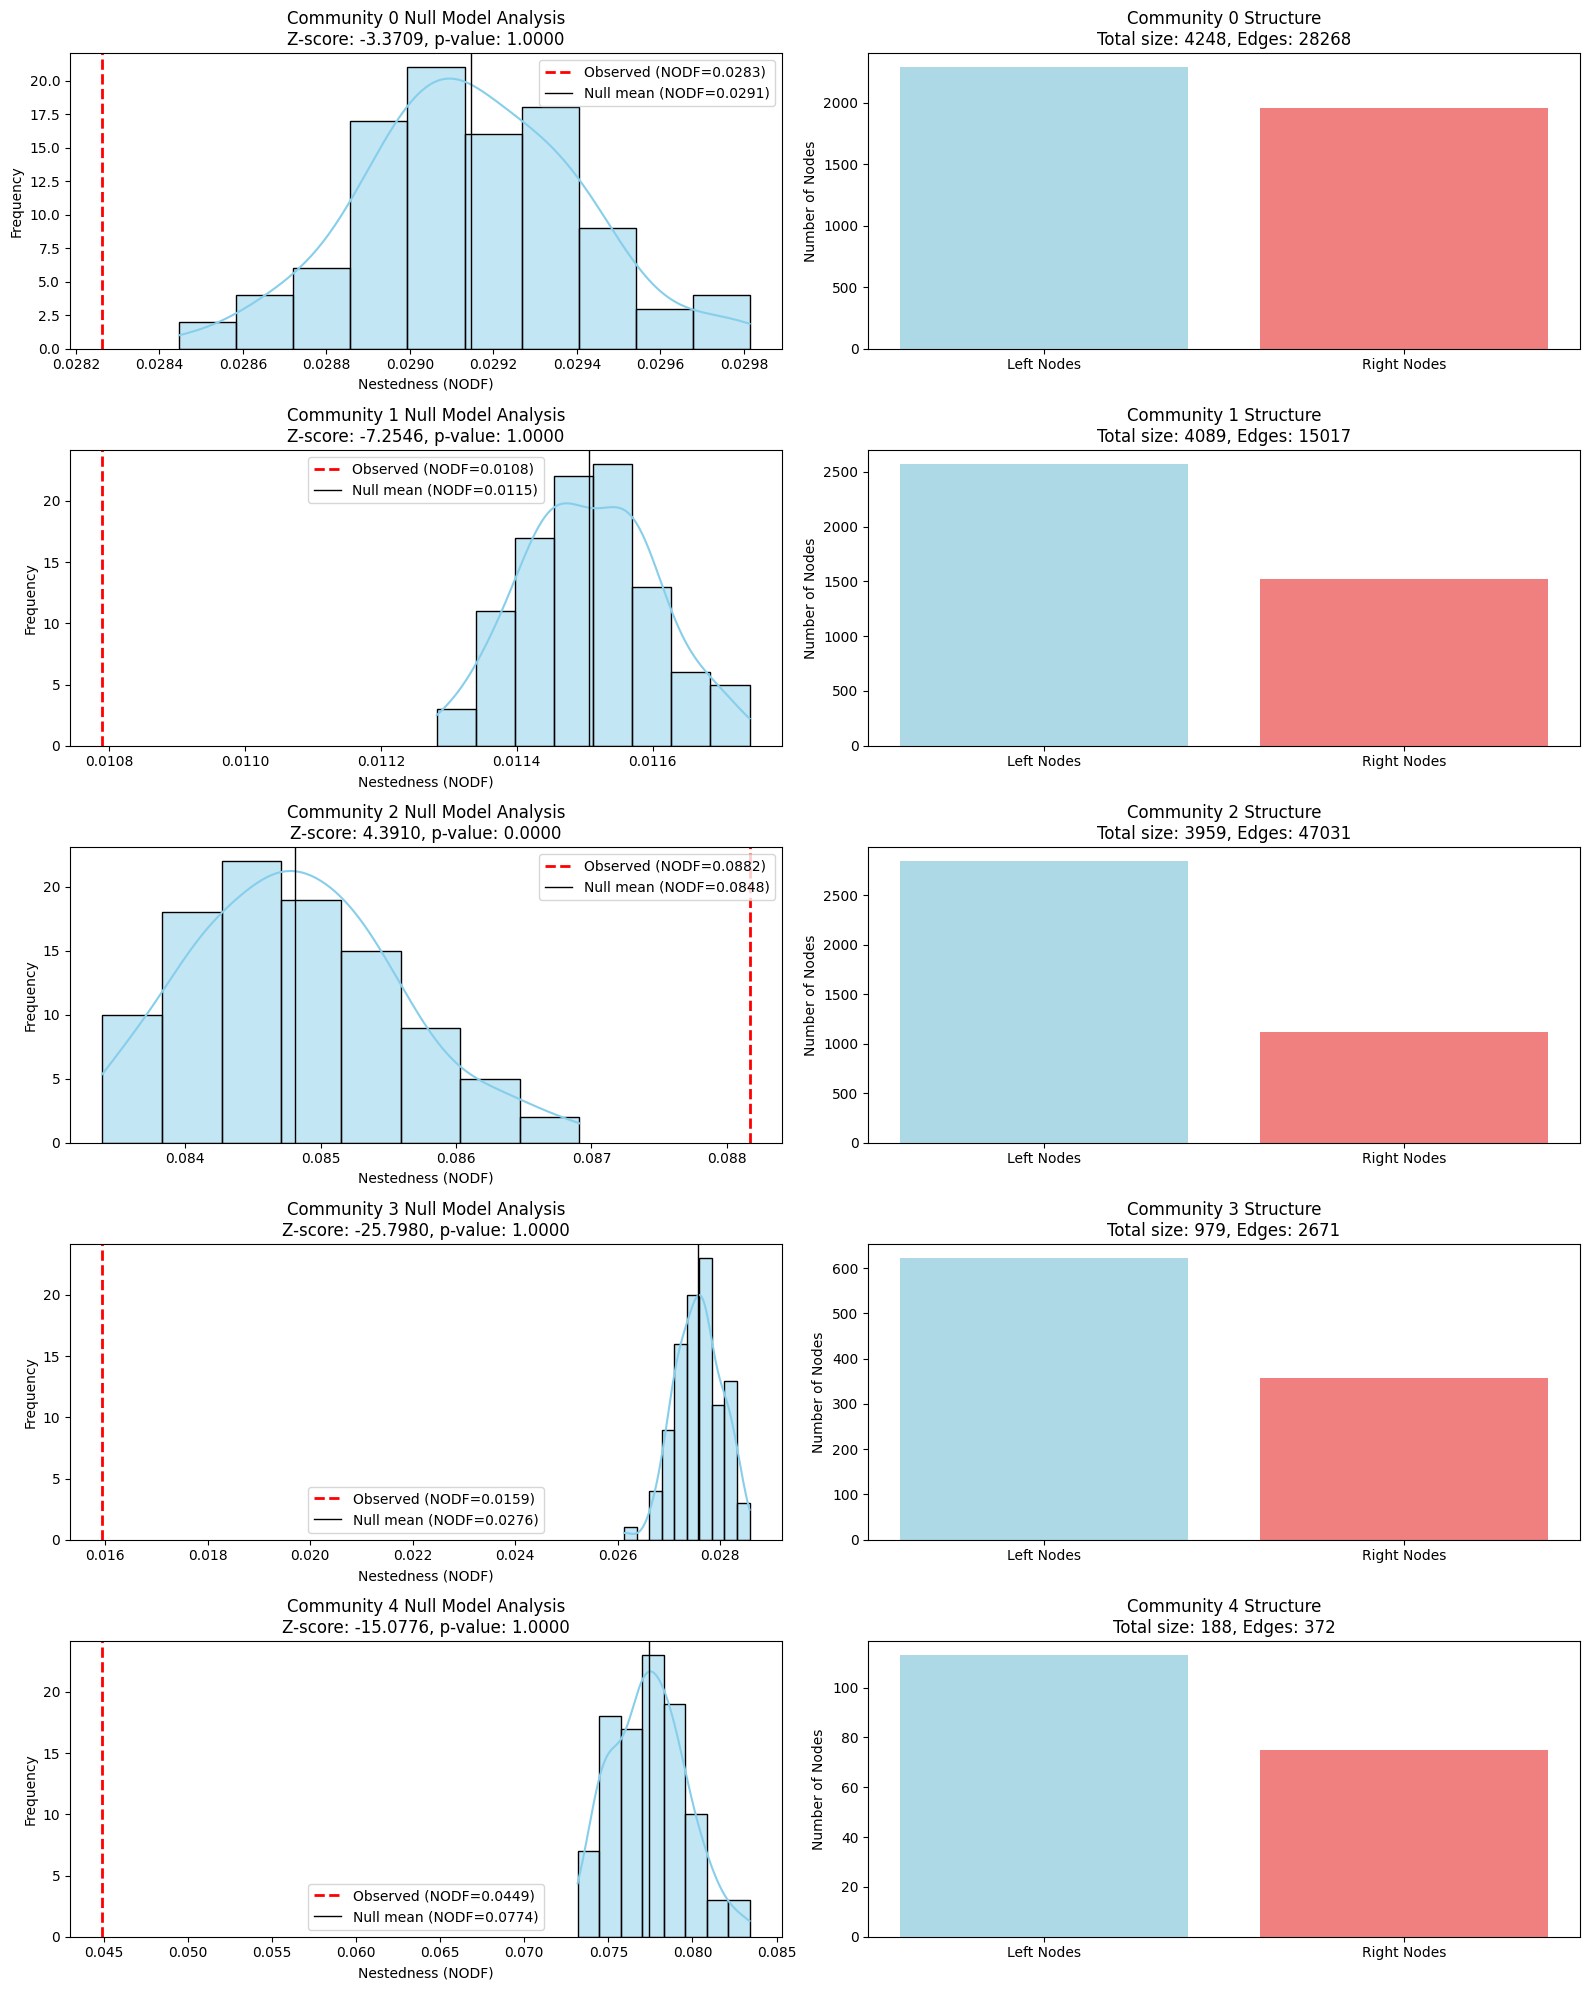
\includegraphics[width=0.8\textwidth]{./assets/null-model-analysis-top-5.png}
\caption{Comparison of observed versus null model nestedness scores for the five largest investor communities. The diagonal line represents equal observed and expected values, with points above the line indicating higher-than-random nestedness. "Left" stands for late stage investors, and "Right" for early stage ones.}
\label{fig:nestedness_comparison}
\end{figure}

\newcommand{\interestingCommunity}{2}
\newcommand{\interestingCommunityNODF}{0.088}
\newcommand{\interestingCommunityPValue}{0.00001}

Community \interestingCommunity{} demonstrates the most pronounced nestedness, exhibiting an NODF score of \interestingCommunityNODF{} with statistical significance of p = \interestingCommunityPValue{}. This hierarchical structure indicates that less-connected investors maintain co-investment relationships with subsets of partners associated with highly-connected investors, creating a hierarchical investment pattern.

Additionally, Community \interestingCommunity{} exhibits an asymmetric composition with a pronounced ratio favoring late-stage investors over early-stage investors. This imbalance contributes to the nested structure by creating hierarchical dependencies between investor types.

The following sections provide detailed characterization of this nested community through comparison with Communities 0 and 1, which serve as contrasting examples of similar-sized but differently structured investor networks.

\subsection{Communities Characterization}

Community boundaries are defined at the node level, meaning each investor belongs to exactly one community. However, edges (investment relationships) can span community boundaries when investors from different communities co-invest in the same startup.

To analyze investment patterns, we classify each syndicated investment as either: (1) intra-community if all participating investors belong to the same community, or (2) cross-community if investors from multiple communities participate together.

Table \ref{tab:investment_distribution} presents the resulting investment distribution across communities.

\begin{table}[htbp]
\centering
\begin{tabular}{|c|c|c|}
\hline
\textbf{Community} & \textbf{Number of Investments} & \textbf{Relative Proportion} \\
\hline
Community 0 & 32,164 & 19.4\% \\
Community 1 & 17,301 & 10.4\% \\
Community 2 & 55,863 & 33.6\% \\
Community 3 & 2,904 & 1.7\% \\
Cross-community & 58,329 & 35.1\% \\
\hline
\textbf{Total} & \textbf{166,561} & \textbf{100\%} \\
\hline
\end{tabular}
\caption{Distribution of syndicated investments across investor communities}
\label{tab:investment_distribution}
\end{table}

The analysis reveals important patterns in investment activity distribution. Community 2, which exhibits significant nestedness, accounts for the largest share of investments (33.6\%), containing approximately 50\% more investments than Community 0 and over three times more than Community 1. This concentration of investment activity within the nested community suggests that hierarchical investor structures may facilitate higher transaction volumes. Notably, cross-community investments represent over one-third of all transactions, indicating substantial interconnectedness across community boundaries.

\subsubsection{Funding Characteristics}

Analysis of funding patterns reveals that the nested Community 2 exhibits substantially higher funding frequency and larger investment amounts compared to the other communities, as demonstrated in Figure \ref{fig:funding_characteristics}.

\todo{Add attachment with statistical proofs}

\begin{figure}[htbp]
\centering
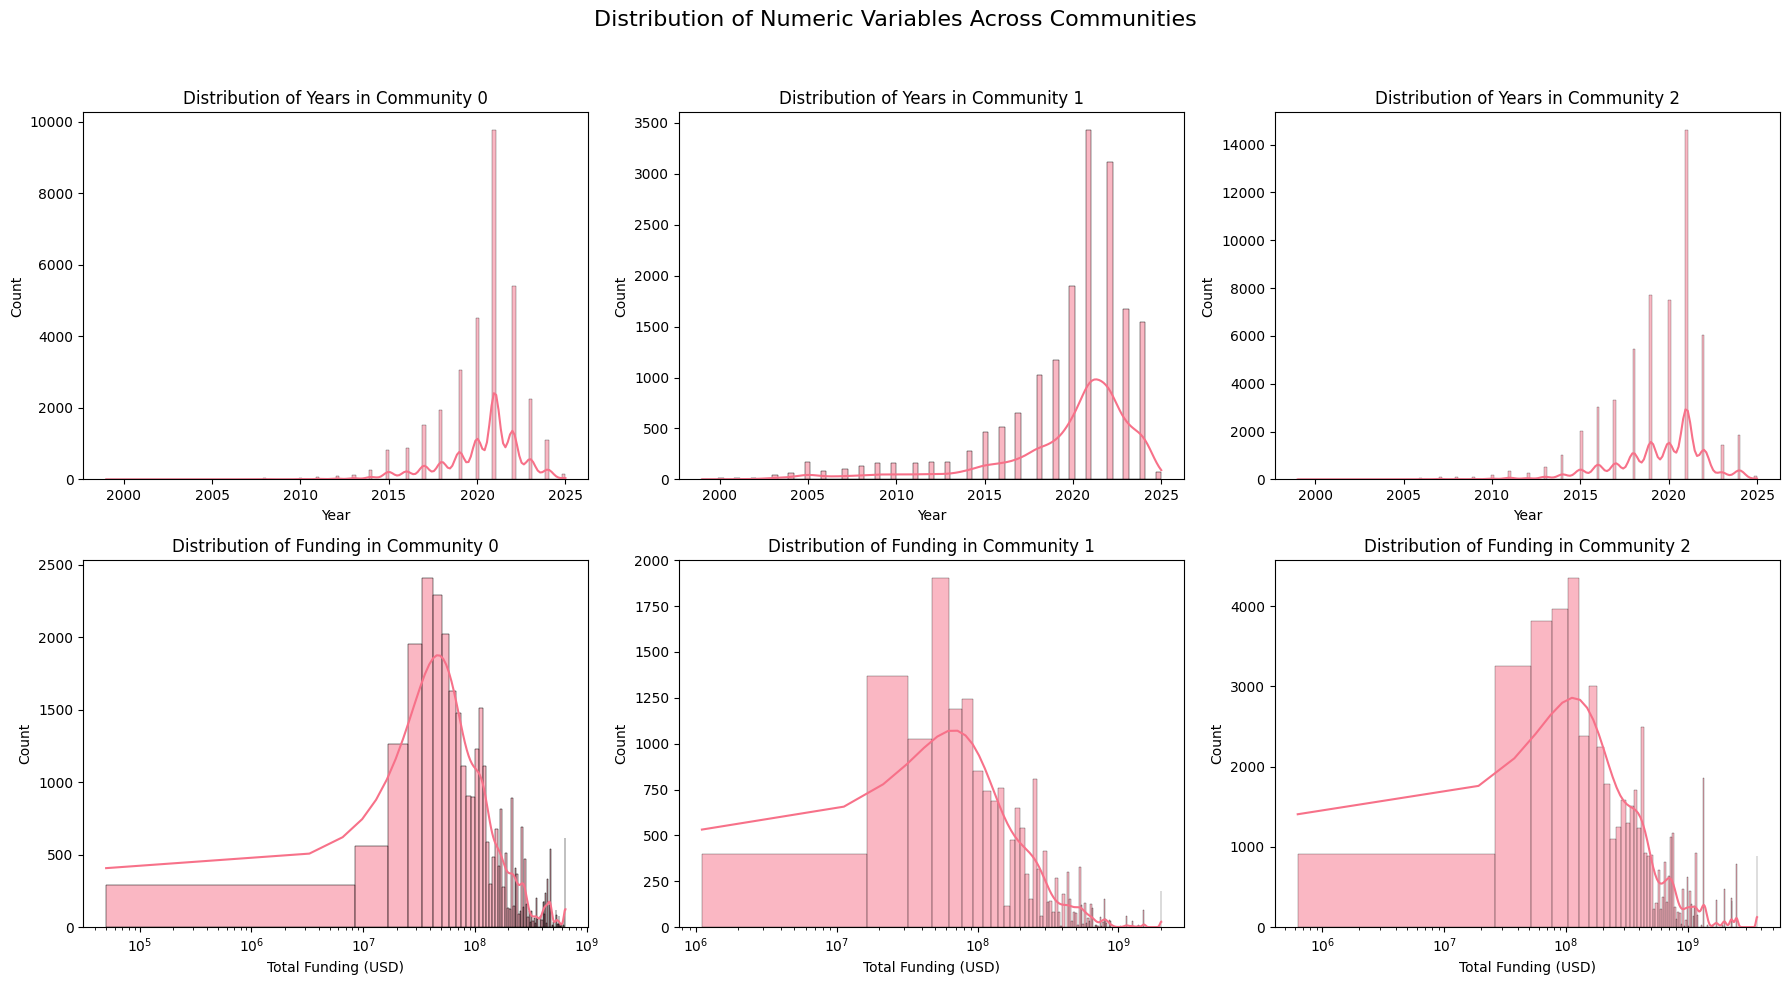
\includegraphics[width=0.8\textwidth]{./assets/funding-characteristics.png}
\caption{Funding characteristics across the three largest investor communities. The analysis reveals systematic differences in investment amounts, round frequency, and funding patterns between communities, with nested structures exhibiting distinct capital deployment strategies compared to randomly organized investor groups.}
\label{fig:funding_characteristics}
\end{figure}

\todo[]{plot a graph of distribtuion of invesments among degrees of investors}

The funding characteristics analysis indicates that nested communities exhibit concentrated capital deployment patterns, with higher-degree investors participating in larger funding rounds while maintaining broader portfolio diversification. This suggests that hierarchical investor organization may create more efficient capital allocation mechanisms compared to randomly structured networks.

Despite superficial similarities between Communities 0 and 2 in terms of size and geographic concentration within the United States, the nested structure in Community 2 appears to confer distinctive advantages. While both communities share comparable scales and American investor bases, Community 2's hierarchical organization enables it to achieve substantially higher transaction volumes (33.6\% vs. 19.4\% of total investments) and more comprehensive funding coverage across all investment stages. This pattern may suggest that nestedness functions as an organizational catalyst, transforming communities with otherwise similar characteristics into more efficient capital deployment networks.

\todo[]{add literature base for this strong assumption}

\subsubsection{Geographic Distribution}

Geographic analysis reveals distinct spatial clustering patterns across the three largest communities. Figure \ref{fig:geographic_distribution} illustrates the asymmetric geographic distributions between early-stage and late-stage investment networks.

\todo[inline]{Better format geographic distribution figure}

\begin{figure}[htbp]
\centering
\begin{subfigure}{0.48\textwidth}
    \centering
    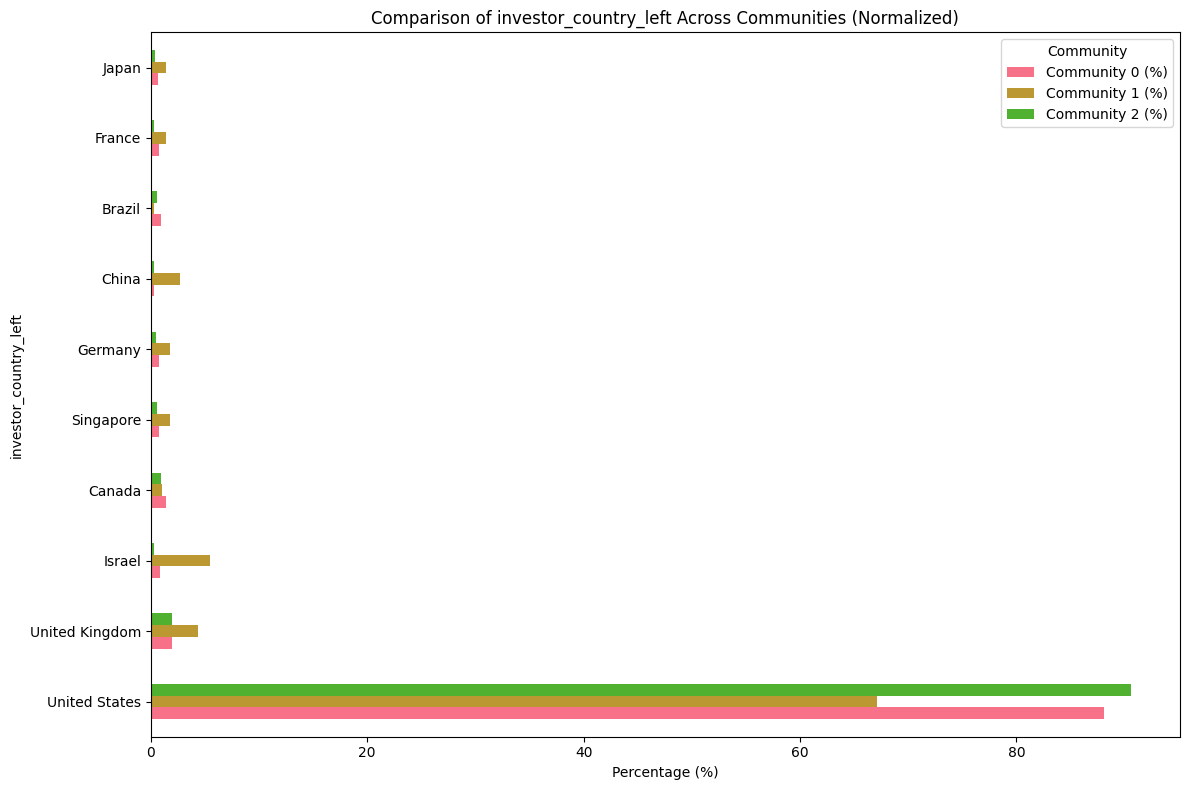
\includegraphics[width=\textwidth]{./assets/investor-left-countries.png}
    \caption{Late-stage investors geographic distribution}
    \label{fig:late_stage_geo}
\end{subfigure}
\hfill
\begin{subfigure}{0.48\textwidth}
    \centering
    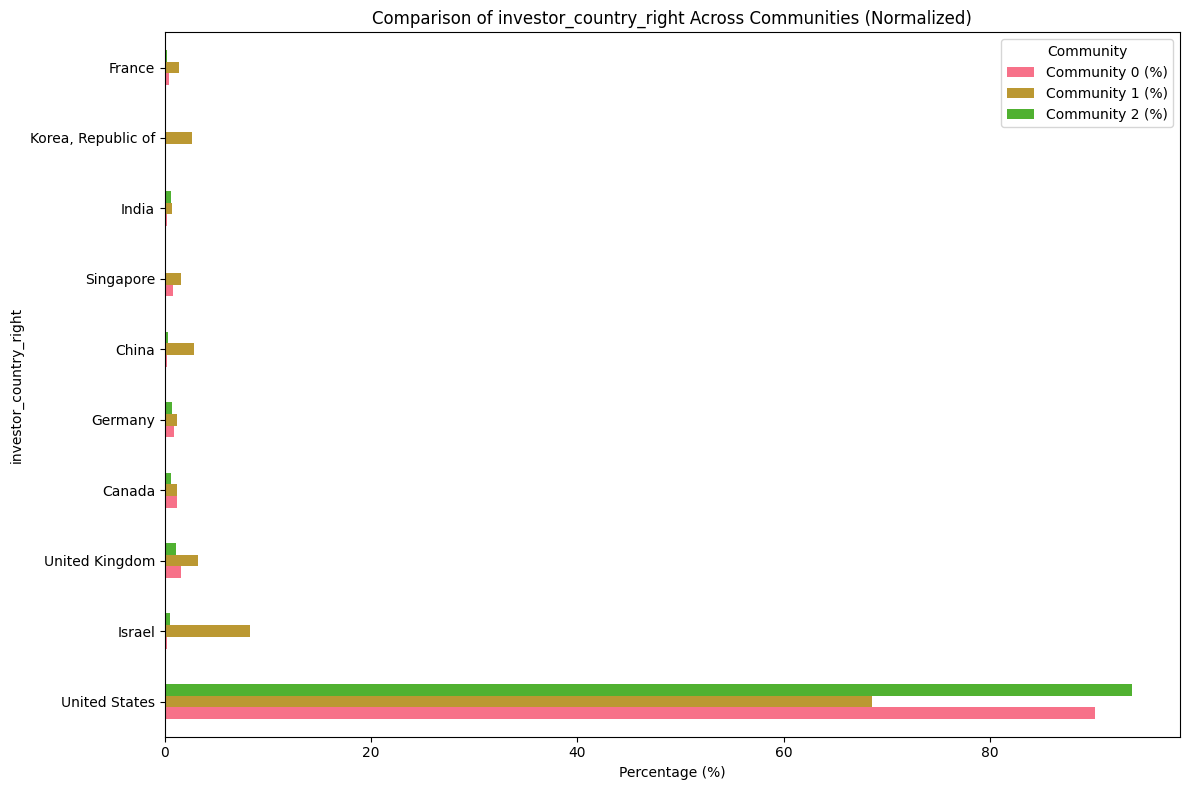
\includegraphics[width=\textwidth]{./assets/investor-right-countries.png}
    \caption{Early-stage investors geographic distribution}
    \label{fig:early_stage_geo}
\end{subfigure}
\caption{Geographic distribution of venture capital investors across the largest communities. The bipartite structure reveals differential geographic clustering between late-stage (left) and early-stage (right) investor networks, with Community 1 exhibiting greater international diversification compared to the U.S.-concentrated Communities 0 and 2.}
\label{fig:geographic_distribution}
\end{figure}

% The geographic distributions exhibit notable asymmetries: late-stage investors demonstrate greater international representation, while early-stage investors show concentrated domestic clustering. This pattern suggests stage-specific geographic preferences that may reflect risk tolerance, regulatory constraints, or information asymmetries across international markets.

Communities 0 and 2 exhibit similar geographic profiles with predominantly American investors, reflecting the dominance of U.S.-based venture capital (important to remember our dataset contains only American startups' investments, which include international investors). However, regional analysis within the United States reveals a striking pattern: Community 2 demonstrates exceptional concentration in California, particularly Silicon Valley, with approximately 50\% more California-based investors than either Community 0 or Community 1 for both late-stage and early-stage investor categories.

This Silicon Valley concentration in the nested Community 2 is particularly significant given the region's status as the world's premier innovation ecosystem. The dominance of California investors in the only statistically nested community suggests a potential relationship between geographic clustering in innovation hubs and the emergence of hierarchical investment structures. This pattern may reflect the dense information networks, frequent face-to-face interactions, and shared risk assessment practices characteristic of Silicon Valley's venture capital community.

In contrast, Community 1 demonstrates significantly greater international diversification, with substantial representation from Israel, the United Kingdom, China, South Korea, Singapore, and France. This international composition in Community 1 may reflect different risk tolerance profiles, regulatory environments, or access to cross-border deal flow compared to the more domestically concentrated communities.

\subsubsection{Investment Stage Preferences}

The investment stage distributions reveal systematic specialization patterns across communities that align with their geographic profiles and transaction volumes. Figure \ref{fig:investment_stage_distribution} demonstrates the distribution patterns of investment types within the bipartite network structure.

\begin{figure}[htbp]
\centering
\begin{subfigure}{0.48\textwidth}
    \centering
    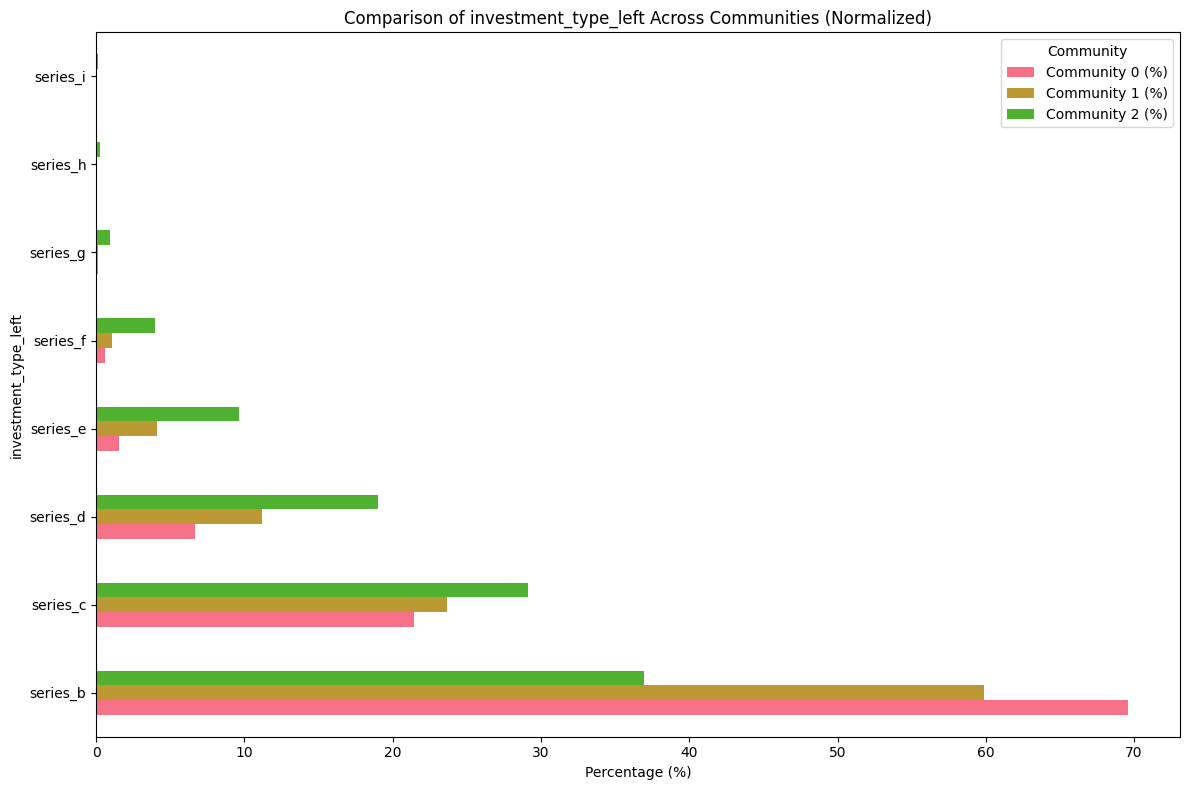
\includegraphics[width=\textwidth]{./assets/late-investment-types-distribution.png}
    \caption{Late-stage investment types distribution}
    \label{fig:late_stage_types}
\end{subfigure}
\hfill
\begin{subfigure}{0.48\textwidth}
    \centering
    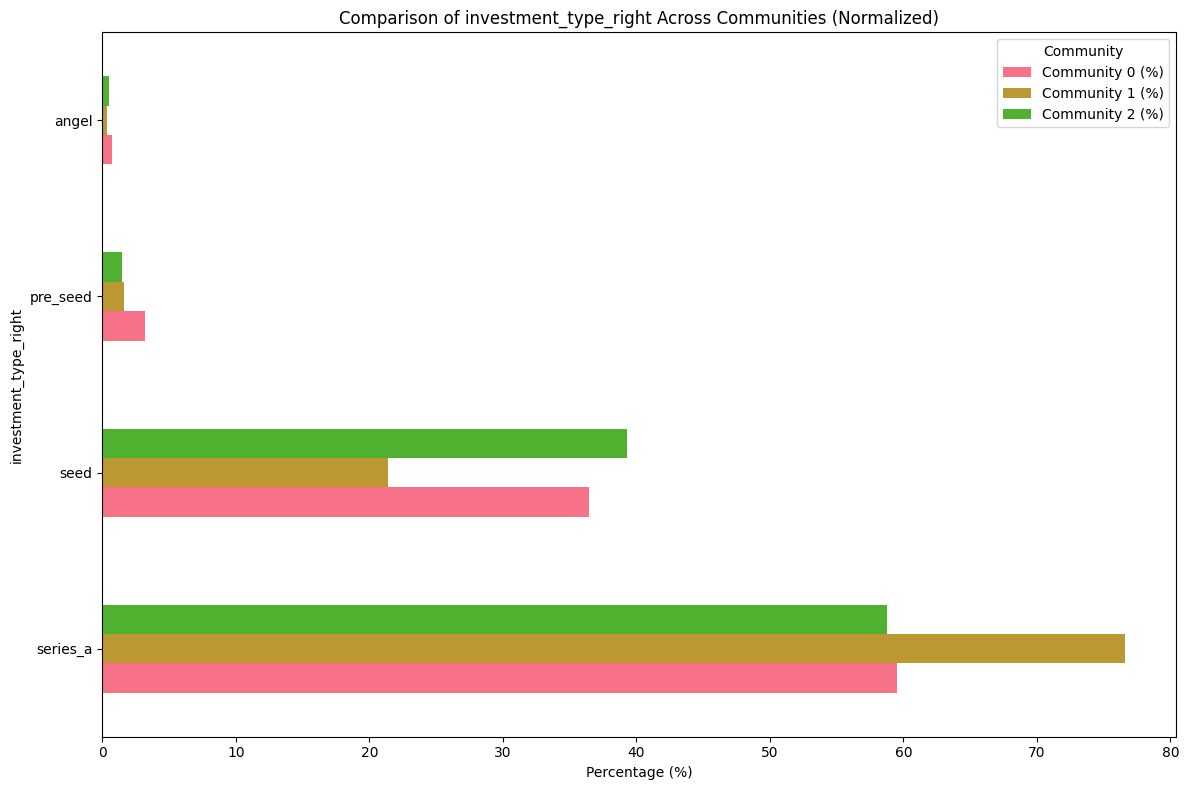
\includegraphics[width=\textwidth]{./assets/early-investment-types-distribution.png}
    \caption{Early-stage investment types distribution}
    \label{fig:early_stage_types}
\end{subfigure}
\caption{Investment stage distribution across the three largest communities. The distribution patterns reveal stage-specific specialization within investor communities.}
\label{fig:investment_stage_distribution}
\end{figure}


\todo[inline]{Comment investment stages distribution}

\textbf{Late-stage investment patterns:} Community 2 dominates Series C and later funding rounds, demonstrating its role in growth-stage capital deployment. Community 1, despite its smaller transaction volume, shows strong representation in Series B and later stages, with participation rates exceeding Community 0 in Series C and beyond. Community 0 exhibits particular strength in Series B rounds while maintaining lower participation in later stages compared to Community 2.

\textbf{Early-stage investment patterns:} Community 2 shows prominence in seed-stage investments while maintaining comparable levels to Community 0 in Series A funding. Both Communities 0 and 2 participate actively in angel and seed rounds, though Community 0 shows relatively higher pre-seed activity. Community 1 demonstrates concentrated focus on Series A investments, aligning with its international profile and suggesting specialization in cross-border early-growth funding.

These stage-specific patterns suggest that the nested structure in Community 2 facilitates participation across the entire funding spectrum, from seed to late-stage rounds, potentially enabling more comprehensive support for portfolio companies throughout their development lifecycle.

\subsubsection{Sectoral Focus}

The sectoral analysis reveals distinct specialization patterns that align with each community's structural and geographic characteristics. Figure \ref{fig:sectoral_distribution} illustrates the distribution of investment focus across technology sectors, demonstrating how different communities exhibit varying degrees of sectoral concentration.

\begin{figure}[htbp]
\centering
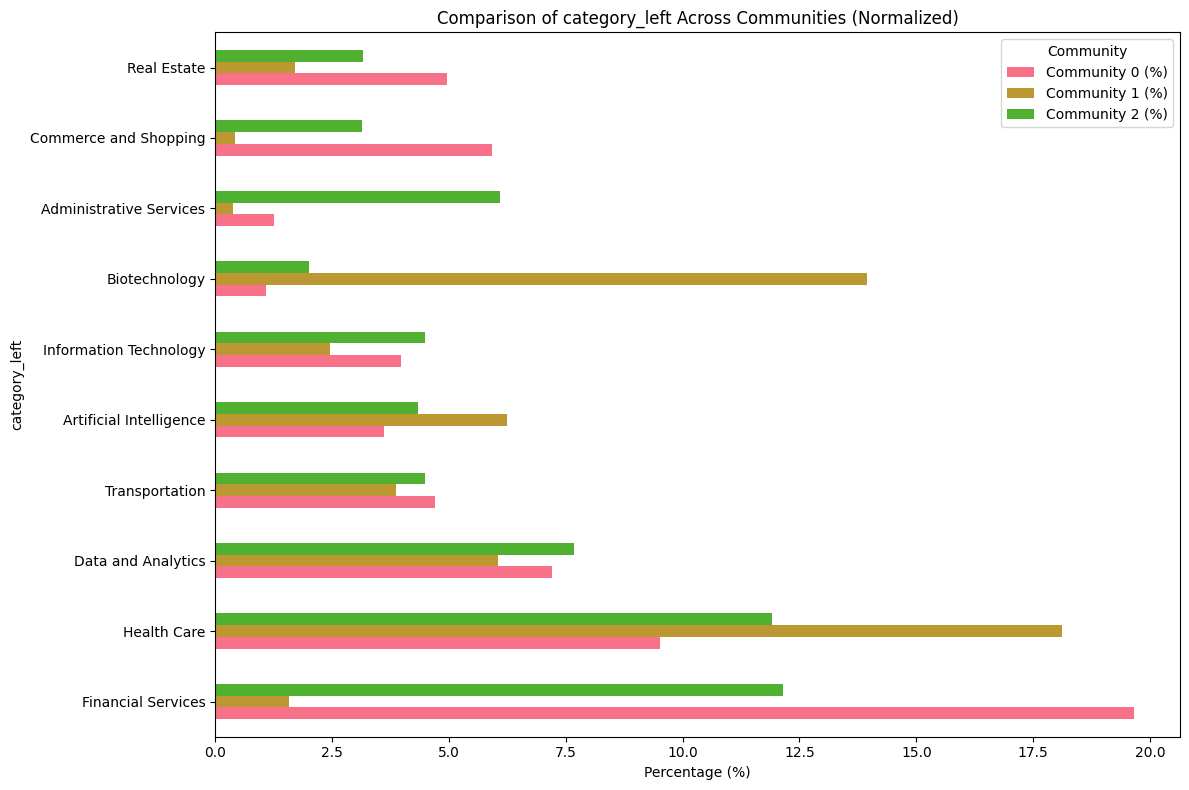
\includegraphics[width=0.8\textwidth]{./assets/sectorial-distribution.png}
\caption{Sectoral distribution across the three largest investor communities. The analysis reveals differential industry focus patterns, with certain communities demonstrating concentrated investment strategies in specific technology sectors while others maintain broader sectoral diversification.}
\label{fig:sectoral_distribution}
\end{figure}

\todo[inline]{Comment sectorial distribution}

\textbf{Community 0:} Concentrates in real estate, commerce and shopping, and financial services, while maintaining standard representation in information technology and artificial intelligence. Notably absent from administrative services and biotechnology, suggesting specialized expertise in consumer-facing and financial technology sectors.

\textbf{Community 1:} Specializes significantly in biotechnology and healthcare, with enhanced artificial intelligence focus compared to other communities. Shows reduced interest in real estate, commerce and shopping, and administrative services. The biotechnology concentration aligns with its international composition, potentially reflecting access to global biotech innovation hubs.

**Community 2:** The nested community exhibits strong representation in administrative services while maintaining comparable levels to Community 0 in information technology and artificial intelligence. Despite its larger transaction volume, it shows lower concentration in real estate and financial services than Community 0, suggesting that nested structure facilitates broader sectoral participation rather than concentrated specialization. This sectoral breadth, combined with the community's Silicon Valley concentration, indicates that nestedness may enable more diversified investment strategies within innovation-rich geographic clusters.

Community 0 serves as an effective structural baseline for comparison with nested Community 2, given their similar geographic profiles and certain sectoral overlaps, while differing significantly in network organization and transaction volumes. The systematic differences observed between these structurally similar communities underscore a potential impact of nested organization on investment behavior and capital deployment efficiency.

\todo[inline]{Add overall comparison}
\todo[inline]{Comment more on funding characteristics}
